\chapter{向量代数}
\section{向量的基本概念}
\subsection{几何概念}
\thispagestyle{empty}
\vspace*{-0.5cm}
\enupdefination[向量相关几何概念]
\begin{enumerate}[]
	\setlength{\itemindent}{3em}
	\setlength{\topsep}{0.01em}
	\setlength{\itemsep}{0.01em}
	\item \quad 
	\begin{figure}[h]
		\centering
		\begin{minipage}{0.8\linewidth}
			\item $\bullet$\quad {\color{dy2}向量\index{XL@向量!XL@向量}}:既有大小又有方向的量. 用符号\boldmath$a,b,c,\cdots ,$\unboldmath 或$\overrightarrow{a},\overrightarrow b$,\\$\overrightarrow{c},\cdots $表示.
			\item $\bullet$\quad {\color{dy2}向量的模\index{XL@向量!XLDM@向量的模}}:一个向量$\overrightarrow{a}$可以用一条有向线段$\overrightarrow{AB}$来表示,那么线段的长度$|AB|$就叫做向量的模(长度).用起点$A$到终点$B$的指向来表示向量量$\overrightarrow{a}$的方向.如图\ref{向量}. 
			\item $\bullet$\quad {\color{dy2}零向量\index{XL@向量!LXL@零向量}}:长度为$0$的向量. 记作$0$. {\color{dy}零向量的方向不确定. }
			\item $\bullet$\quad {\color{dy2}单位向量\index{XL@向量!DWXL@单位向量}}:长度为$1$的向量. 与$\overrightarrow{a}$同向的单位向量记作$\overrightarrow{a^0}$
			\item $\bullet$\quad {\color{dy2}反向量\index{XL@向量!FXL@反向量}}:与原向量大小相等方向相反的向量. 记作$-\overrightarrow{a}$.
		\end{minipage}%
		\hfill
		\begin{minipage}{0.2\linewidth}
			\centering
			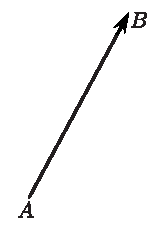
\includegraphics[width=0.9\linewidth]{picture/C-1/1.1/xl1}
			\caption{向量的表示}
			\label{向量}
		\end{minipage}%
	\end{figure}
\end{enumerate}

\subsection{解析概念}
\vspace*{-0.5cm}
\enupdefination[向量解析相关概念]
\begin{enumerate}[]
	\setlength{\itemindent}{3em}
	\setlength{\topsep}{0.01em}
	\setlength{\itemsep}{0.01em}
	\item 
	\item $\bullet$\quad{\color{dy2}基\index{XL@向量!J@基}}:空间中任意三个有次序的不共面的向量$\overrightarrow{e_1},\overrightarrow{e_2},\overrightarrow{e_3}$称为空间中的一组基.
	\item $\bullet$\quad{\color{dy2}坐标\index{XL@向量!ZB@坐标}}:对于空间中任一向量$\overrightarrow m$,若
	\begin{equation}
		\overrightarrow{m}=x\overrightarrow{e_1}+y\overrightarrow{e_2}+z\overrightarrow{e_3}
	\end{equation}
	则把有序三元实数组$(x,y,z)$称为$\overrightarrow{m}$在基$\overrightarrow{e_1},\overrightarrow{e_2},\overrightarrow{e_3}$中的坐标.
	\item $\bullet$\quad{\color{dy2}定位向量(矢径)\index{XL@向量!DWXL@定位向量}}:在空间中取定一个点$O$以后,任意一个点$M$与向量$\overrightarrow{OM}$一一对应,因此称$\overrightarrow{OM}$为点$M$的定位向量(矢径\index{XL@向量!SJ@矢径}). 
\end{enumerate}

	\begin{figure}[h]
		\sj 
\defination[坐标系相关概念]
\end{figure}

\begin{enumerate}[]
	\setlength{\itemindent}{3em}
	\setlength{\topsep}{0.01em}
	\setlength{\itemsep}{0.01em}
	\begin{figure}[h]
		\begin{minipage}{0.6\linewidth}
			\item $\bullet$\quad{\color{dy2}仿射坐标系}\index{FSZBX@仿射坐标系!FSZBX@仿射坐标系}:空间中的一个点$O$和一组基$\overrightarrow{e_1},\overrightarrow{e_2},\overrightarrow{e_3}$合在一起称为空间的一个{\color{dy2}仿射标架}或{\color{dy2}仿射坐标系}\index{FSZBX@仿射坐标系!FSBJ@仿射标架},记作$[O;\overrightarrow{e_1},\overrightarrow{e_2},\overrightarrow{e_3}]$,其中$O$称为{\color{dy2}原点}\index{FSZBX@仿射坐标系!YD@原点}. {\color{dy}特别地,当仿射坐标系的基向量两两垂直时,称为直角坐标系\index{FSZBX@仿射坐标系!ZJZBX@直角坐标系}}.
			\item $\bullet$\quad{\color{dy2}坐标轴\index{FSZBX@仿射坐标系!ZBJ@坐标轴}}:过原点$O$,且分别以$\overrightarrow{e_1},\overrightarrow{e_2},\overrightarrow{e_3}$为方向得有向直线分别称为$x$轴,$y$轴,$z$轴,统称为{\color{dy2}坐标轴}. 
			\item$\bullet$\quad {\color{dy2}坐标平面\index{FSZBX@仿射坐标系!ZBPM@坐标平面}}:由每两根坐标轴决定的平面称为{\color{dy2}坐标平面},分别为$xOy,yOz,zOx$平面. 
			\item $\bullet$\quad{\color{dy2}卦限\index{FSZBX@仿射坐标系!GX@卦限}}:坐标平面把空间分成八个部分,称为八个{\color{dy2}卦限}. 如图\ref{八卦}. 
			\item $\bullet$\quad{\color{dy2}左右手系}:将右手的拇指和食指分别指着$x$轴,$y$轴,如果中值所指的方向与$z$轴方向在$xOy$平面同侧,则称此坐标系为{\color{dy2}右手系\index{FSZBX@仿射坐标系!YSX@右手系}},否则称为{\color{dy2}左手系\index{FSZBX@仿射坐标系!ZSX@左手系}}. 
		\end{minipage}
		\hfill
		\begin{minipage}{0.4\linewidth}
			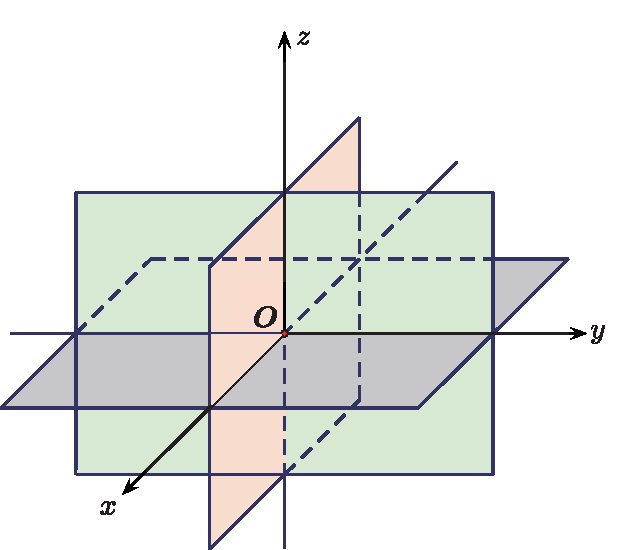
\includegraphics[scale=0.75]{picture/C-1/1.1/BG.pdf}
			\caption{仿射坐标系及其八卦}
			\label{八卦}
		\end{minipage}
	\end{figure}
\end{enumerate}
\jg
\jg

\subsection{方向角与方向余弦}
\tdefination[向量的夹角]\index{XL@向量!XLDJJ@向量的夹角}
设有两个非零向量$\overrightarrow{a}$,$\overrightarrow{b}$,任取空间中一点$O$ ,作$\overrightarrow{OA}=\overrightarrow{a},\overrightarrow{OB}=\overrightarrow{b}$,规定$0\le \varphi=\angle AOB\le \pi $,那么$\angle AOB$称为向量$\overrightarrow{a}$,$\overrightarrow{b}$的夹角,即$0\le\left\langle \overrightarrow{a},\overrightarrow{b}\right\rangle =\left\langle \overrightarrow{b},\overrightarrow{a}\right\rangle =\varphi\le \pi $.

\begin{figure}[h]
	\begin{minipage}{0.5\linewidth}
		\centering 
		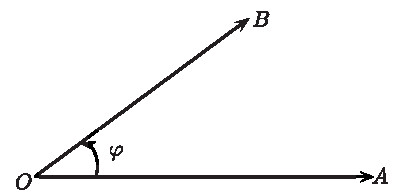
\includegraphics[width=0.9\linewidth]{picture/C-1/1.1/angle.pdf}
		\caption{向量的夹角}
	\end{minipage}
	\hfill
	\begin{minipage}{0.5\linewidth}
		\centering 
		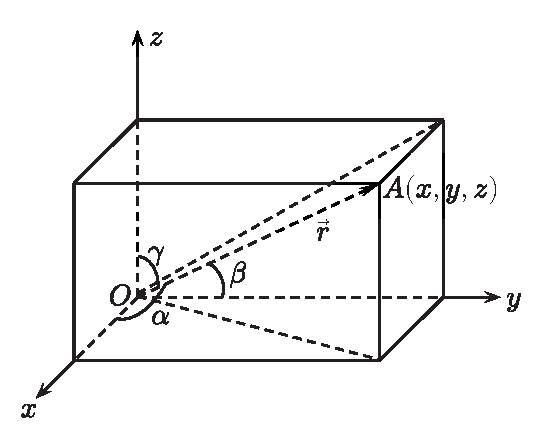
\includegraphics[width=0.9\linewidth]{picture/C-1/1.1/angle2.pdf}
		\caption{方向角与方向余弦}
	\end{minipage}
\end{figure}
\newpage 
\defination[方向角与方向余弦]\index{FSZBX@仿射坐标系!FXJYFXYX@方向角与方向余弦}
\quad 记非零向量$\overrightarrow{r}$与三条坐标轴($x$轴,$y$轴,$z$轴)的夹角分别为$\alpha ,\beta ,\gamma$.称为向量$\overrightarrow{r}$的方向角.设$\overrightarrow{r}=\overrightarrow{OA}=(x,y,z)$,若$\sqrt{x^2+y^2+z^2}\ne 0,$则
\begin{equation*}
	\cos \alpha =\frac{x}{|\overrightarrow{r}|}=\frac{x}{	\sqrt{x^2+y^2+z^2}}\qquad 
	\cos \beta =\frac{y}{|\overrightarrow{r}|}=\frac{y}{	\sqrt{x^2+y^2+z^2}}\qquad
	\cos \gamma =\frac{z}{|\overrightarrow{r}|}=\frac{z}{	\sqrt{x^2+y^2+z^2}}
\end{equation*}

\section{向量的基本运算}
\subsection{线性运算}\index{XXYS@线性运算!XXYS@线性运算}
\begin{enumerate}
	\setlength{\itemindent}{0em}
	\setlength{\topsep}{0.01em}
	\setlength{\itemsep}{0.01em}
	\item {\color{dy}加(减)法\index{XXYS@线性运算!JF@加法}}
	\begin{enumerate}[(1)]
		\setlength{\topsep}{0.01em}
		\setlength{\itemsep}{0.01em}
		\item {\color{dy2}几何表示}
		\begin{enumerate}[]
					\setlength{\itemindent}{1em} 
			\setlength{\topsep}{0.01em}
			\setlength{\itemsep}{0.01em}
			\item 对于向量 $\overrightarrow a,\overrightarrow b$,作有向线段 ,作有向线段 $\overrightarrow {AB}$表示 $\overrightarrow a$,作 $\overrightarrow {BC}$表示 $\overrightarrow b$,则把有向线段 $\overrightarrow {AC}$表示的向量 $\overrightarrow c$称为 向量$\overrightarrow a$与$\overrightarrow b$的和 .向量加法运算规则在几何上称为向量加法运算规则在几何上称为{\color{dy}三角形法则\index{XXYS@线性运算!JF@加法!SJXFZ@三角形法则}}或{\color{dy}平行四边形法则\index{XXYS@线性运算!JF@加法!PXSBXFZ@平行四边形法则}} .如图\ref{向量加法}.
			\begin{figure}[h]
				\centering
				\subfigure[三角形法则]{
					\begin{minipage}[t]{0.5\linewidth}
						\centering
						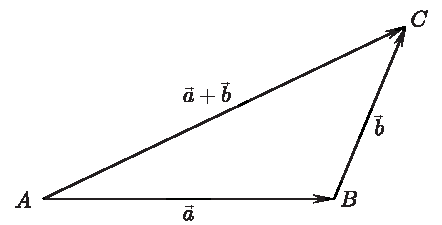
\includegraphics[width=0.9\linewidth]{picture/C-1/1.2/JF2}
						%\caption{fig1}
					\end{minipage}%
				}%
				\subfigure[平行四边形法则]{
					\begin{minipage}[t]{0.5\linewidth}
						\centering
						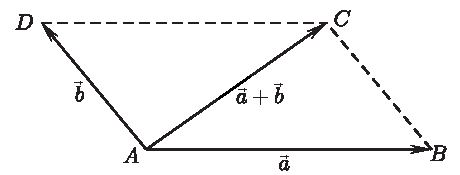
\includegraphics[width=0.9\linewidth]{picture/C-1/1.2/JF1}
						%\caption{fig2}
					\end{minipage}%
				}%
				
				\centering
				\caption{向量的加法法则}
				\label{向量加法}
			\end{figure}
		\end{enumerate}
		\item {\color{dy2}坐标表示}
		\begin{enumerate}[]
					\setlength{\itemindent}{1em} 
			\setlength{\topsep}{0.01em}
			\setlength{\itemsep}{0.01em}
			\item 设$\overrightarrow a = (x_1,y_1,z_1),\overrightarrow b = (x_2,y_2,z_2)$,则$\overrightarrow a +\overrightarrow b =(x_1+x_2,y_1+y_2,z_1+z_2)$
		\end{enumerate}
		\item {\color{dy2}运算律}
		\begin{enumerate}
					\setlength{\itemindent}{1em} 
			\setlength{\topsep}{0.01em}
			\setlength{\itemsep}{0.01em}
			\begin{minipage}{0.6\linewidth}
				\item 交换律:$\overrightarrow a+\overrightarrow b =\overrightarrow b+\overrightarrow a$
				\item 结合律:$\left( \overrightarrow a+\overrightarrow b\right)  +\overrightarrow  c= \overrightarrow a+\left( \overrightarrow b  +\overrightarrow  c\right) $
				\item 任意向量$\overrightarrow{a}$,有$\overrightarrow{a}+\overrightarrow{0}$
				\item 任意向量$\overrightarrow{a}$,有$\overrightarrow{a}-\overrightarrow{a}=\overrightarrow{0}$
				\item 向量的减法:$\overrightarrow{a} - \overrightarrow{b} =\overrightarrow{a} +(- \overrightarrow{b} )$
			\end{minipage}
			\hfill
			\begin{minipage}{0.4\linewidth}
				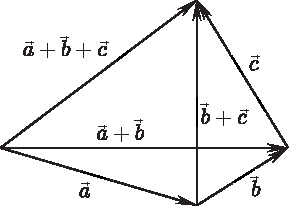
\includegraphics[width=0.9\linewidth]{picture/C-1/1.2/JF3}
			\end{minipage}
		\end{enumerate}
	\end{enumerate}
\newpage
	\item {\color{dy}数乘\index{XXYS@线性运算!SC@数乘}}
	\begin{enumerate}[(1)]
		\setlength{\topsep}{0.01em}
		\setlength{\itemsep}{0.01em}
		\item{\color{dy2}几何表示}
		\begin{enumerate}
			实数$\lambda$与向量$\overrightarrow a$的乘积定义为一个向量$\lambda \overrightarrow{a}$它的长度为
			\begin{equation}
				\left| \lambda \overrightarrow{a}\right| =|\lambda |\cdot \left| \overrightarrow{a}\right|
			\end{equation} 
			当 $\lambda >0$时它的方向与 $\overrightarrow{a}$相同,当 $\lambda <0$时它的方向与 $\overrightarrow{a}$相反 .
		\end{enumerate}
		\item {\color{dy2}坐标表示}
		\begin{enumerate}[]
					\setlength{\itemindent}{1em} 
			\setlength{\topsep}{0.01em}
			\setlength{\itemsep}{0.01em}
			\item 设$\overrightarrow a = (x,y,z)$,则$\lambda\overrightarrow{a}=(\lambda x,\lambda y,\lambda z)$
		\end{enumerate}
		\item{\color{dy2} 运算律}
		\begin{enumerate}
					\setlength{\itemindent}{1em} 
			\setlength{\topsep}{0.01em}
			\setlength{\itemsep}{0.01em}
			\item 结合律:$\lambda (\mu \overrightarrow{a})=(\lambda \mu )\overrightarrow{a}$
			\item 分配律:$(\lambda + \mu )\overrightarrow{a}=\lambda \overrightarrow{a}+\mu \overrightarrow{a} , \qquad \lambda(\overrightarrow{a}+\overrightarrow{b})=\lambda \overrightarrow{a}+\lambda \overrightarrow{b}.$
		\end{enumerate}
	\end{enumerate}
\end{enumerate}
\subsection{线性组合}
\tdefination[线性组合]\index{XXXGX@线性相关性!XXZH@线性组合}
一般地,设 $\overrightarrow {a_1},\overrightarrow {a_2},\cdots ,\overrightarrow {a_m}$是一组向量, $k_1,k_2,\cdots ,k_m$是一组实数,称向量 $k_1\overrightarrow{ a_1},k_2\overrightarrow {a_2},\cdots ,k_m\overrightarrow{ a_m}$为该向量组的一个 {\color{dy}线性组合},称$k_1,k_2,\cdots ,k_m$为这个 {\color{dy}线性组合的系数\index{XXXGX@线性相关性!XXZHDXS@线性组合的系数}}. 


\adddefination[线性相关性]\index{XXXGX@线性相关性!XXXGX@线性相关性}
一般地,设 $\overrightarrow {a_1},\overrightarrow {a_2},\cdots ,\overrightarrow {a_m}$是一组向量,如果存在 一组不全为零的实数$k_1,k_2,\cdots ,k_m$使得:
\begin{equation}
	k_1\overrightarrow{a_1}+k_2\overrightarrow{a_2}+\cdots +k_m\overrightarrow{a_m}=0
	\label{线性相关}
\end{equation}
那么称向量$\overrightarrow {a_1},\overrightarrow {a_2},\cdots ,\overrightarrow {a_m}$ {\color{dy}线性相关}\index{XXXGX@线性相关性!XXXG@线性相关}. 否则称向量组为{\color{dy}线性无关\index{XXXGX@线性相关性!XXWG@线性无关}}.\\
\quad 向量线性相关性的几何意义:线性相关性与向量是否在同一个向量空间等价. 在二阶和三阶向量空间中,向量是否线性相关代表着向量是否共线或共面. 
\jg
\jg
\subsection{内积}\index{NJ@内积}
\begin{enumerate}[1.]
			\setlength{\itemindent}{0em} 
	\setlength{\topsep}{0.01em}
	\setlength{\itemsep}{0.01em}
	\item {\color{dy2}几何表示}
	\begin{enumerate}[]
				\setlength{\itemindent}{1.5em} 
		\setlength{\topsep}{0.01em}
		\setlength{\itemsep}{0.01em}
		\item \begin{equation}
			\overrightarrow{a} \cdot \overrightarrow{b}=|\overrightarrow{a}|\cdot |\overrightarrow{b}| \cos \left\langle \overrightarrow{a},\overrightarrow{b}	\right\rangle 
		\end{equation}
	\end{enumerate}
	\newpage
	\item {\color{dy2}坐标表示}
	\begin{enumerate}[]
				\setlength{\itemindent}{1.5em} 
		\setlength{\topsep}{0.01em}
		\setlength{\itemsep}{0.01em}
		\item 设在仿射标架$[O,\overrightarrow{e_1},\overrightarrow{e_2},\overrightarrow{e_3}]$中$\overrightarrow{a},\overrightarrow{b}$的坐标分别为:$(a_1,a_2,a_3),(b_1,b_2,b_3)$,则
		\begin{equation}
			\begin{aligned}
				\overrightarrow{a} \cdot   \overrightarrow{b}&=(a_1\overrightarrow{e_1}+a_2\overrightarrow{e_2}+a_3\overrightarrow{e_3})\cdot   (b_1\overrightarrow{e_1}+b_2\overrightarrow{e_2}+b_3\overrightarrow{e_3})\\
				&=a_1b_1\cdot  \left[\overrightarrow{e_1}\cdot   \overrightarrow{e_1}\right]+a_1b_2\cdot  \left[\overrightarrow{e_1}\cdot   \overrightarrow{e_2}\right]+a_1b_3\cdot  \left[\overrightarrow{e_1}\cdot  \overrightarrow{e_3}\right]\\
				&\,\,+a_2b_1\cdot  \left[\overrightarrow{e_2}\cdot   \overrightarrow{e_1}\right]+a_2b_2\cdot  \left[\overrightarrow{e_2}\cdot   \overrightarrow{e_2}\right]+a_2b_3\cdot  \left[\overrightarrow{e_2}\cdot  \overrightarrow{e_3}\right]\\
				&\,\,+a_3b_1\cdot  \left[\overrightarrow{e_3}\cdot   \overrightarrow{e_1}\right]+a_3b_2\cdot  \left[\overrightarrow{e_3}\cdot   \overrightarrow{e_2}\right]+a_3b_3\cdot  \left[\overrightarrow{e_3}\cdot   \overrightarrow{e_3}\right]
			\end{aligned}
		\end{equation}
		\qquad 因此,我们要知道两个向量的内积,只需要知道向量$\overrightarrow{e_1},\overrightarrow{e_2},\overrightarrow{e_3}$的内积(九个数)即可,这九个数称为{\color{dy}仿射标架$[O,\overrightarrow{e_1},\overrightarrow{e_2},\overrightarrow{e_3}]$的度量参数\index{FSZBX@仿射坐标系!DLCS@度量参数}}. \\
		\hspace*{2em}特别地,当仿射坐标系的基向量两两垂直时,即为直角坐标系时,内积表达式可写为
		\begin{equation}
			\overrightarrow{a} \cdot \overrightarrow{b}=a_1b_1+a_2b_2+a_3b_3.
		\end{equation}
	\end{enumerate}
	\item {\color{dy2}运算律}
	\begin{enumerate}[i.]
				\setlength{\itemindent}{1.5em} 
		\setlength{\topsep}{0.01em}
		\setlength{\itemsep}{0.01em}
		\item 对称性:$\overrightarrow{a}\cdot \overrightarrow{b}=\overrightarrow{b}\cdot \overrightarrow{a}.$
		\item 数线性:$(\lambda\overrightarrow{a})\cdot \overrightarrow{b}=\overrightarrow{a}\cdot (\lambda \overrightarrow{b}).$
		\item 向量线性:$(\overrightarrow{a}+\overrightarrow{b})\cdot \overrightarrow{c}=\overrightarrow{a}\cdot \overrightarrow{c}+\overrightarrow{b}\cdot\overrightarrow{c}.$
	\end{enumerate}
\end{enumerate}
\jg
\jg
\subsection{外积}\index{WJ@外积}
\begin{enumerate}[1.]
			\setlength{\itemindent}{0em} 
	\setlength{\topsep}{0.01em}
	\setlength{\itemsep}{0.01em}
	\item {\color{dy2}几何表示}\vspace{0.25cm}
	\begin{enumerate}[]
				\setlength{\itemindent}{1.5em} 
		\setlength{\topsep}{0.01em}
		\setlength{\itemsep}{0.01em}
		\begin{figure}[htb]
			\begin{minipage}{0.6\linewidth}
				\item 两个向量$\overrightarrow{a},\overrightarrow{b}$的外积仍然是一个向量,它的长度为
				\begin{equation}
					\left|\overrightarrow{a}\times\overrightarrow{b} \right| =|\overrightarrow{a}|\cdot |\overrightarrow{b}|\sin \left\langle \overrightarrow{a},\overrightarrow{b}\right\rangle 
				\end{equation}
				\item 它的方向为与$\overrightarrow{a},\overrightarrow{b}$构成的平面垂直,右手螺旋为逆时针,则垂直该平面向上;右手螺旋为顺时针,则垂直该平面向下. 
				\item {\color{dy}几何意义}\label{外积的几何意义} :$\left|\overrightarrow{a}\times\overrightarrow{b} \right|$代表的是分别以$\overrightarrow{a},\overrightarrow{b}$为邻边的平行四边形的面积. 如图\ref{外积}.
			\end{minipage}
			\hfill
			\begin{minipage}{0.4\linewidth}
				\centering
				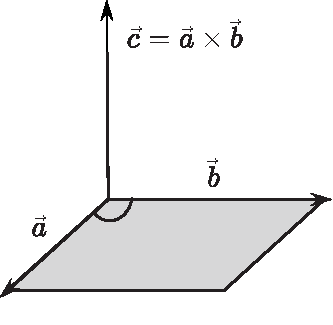
\includegraphics[width=0.7\linewidth]{picture/C-1/1.2/WJ.pdf}
				\caption{外积的几何意义}
				\label{外积}
			\end{minipage}
		\end{figure}
	\end{enumerate}
	\newpage
	\item {\color{dy2}坐标表示}
	\begin{enumerate}[]
				\setlength{\itemindent}{1.5em} 
		\setlength{\topsep}{0.01em}
		\setlength{\itemsep}{0.01em}
		\item 设在仿射标架$[O,\overrightarrow{e_1},\overrightarrow{e_2},\overrightarrow{e_3}]$中$\overrightarrow{a},\overrightarrow{b}$的坐标分别为:$(a_1,a_2,a_3),(b_1,b_2,b_3)$,则
		\begin{equation}
			\begin{aligned}
				\overrightarrow{a} \times \overrightarrow{b}&=(a_1\overrightarrow{e_1}+a_2\overrightarrow{e_2}+a_3\overrightarrow{e_3})\times (b_1\overrightarrow{e_1}+b_2\overrightarrow{e_2}+b_3\overrightarrow{e_3})\\
				&=a_1b_1\cdot  \left[\overrightarrow{e_1}\times \overrightarrow{e_1}\right]+a_1b_2\cdot  \left[\overrightarrow{e_1}\times \overrightarrow{e_2}\right]+a_1b_3\cdot  \left[\overrightarrow{e_1}\times\overrightarrow{e_3}\right]\\
				&\,\, +a_2b_1\cdot  \left[\overrightarrow{e_2}\times \overrightarrow{e_1}\right]+a_2b_2\cdot  \left[\overrightarrow{e_2}\times \overrightarrow{e_2}\right]+a_2b_3\cdot  \left[\overrightarrow{e_2}\times\overrightarrow{e_3}\right]\\
				&\,\,  +a_3b_1\cdot  \left[\overrightarrow{e_3}\times \overrightarrow{e_1}\right]+a_3b_2\cdot  \left[\overrightarrow{e_3}\times \overrightarrow{e_2}\right]+a_3b_3\cdot  \left[\overrightarrow{e_3}\times \overrightarrow{e_3}\right]\\
				&=\left( a_1b_2-a_2b_1\right)\cdot \left[\overrightarrow{e_1}\times \overrightarrow{e_2}\right]+\left(a_3b_1-a_1b_3\right)\cdot \left[\overrightarrow{e_3}\times \overrightarrow{e_1}\right]+\left(a_2b_3-a_3b_2\right)\cdot \left[\overrightarrow{e_2}\times \overrightarrow{e_3}\right] \\
				&=\begin{array}{|ccc|}
					\left[\overrightarrow{e_1}\times \overrightarrow{e_2}\right]&\left[\overrightarrow{e_3}\times \overrightarrow{e_1}\right]  &\left[\overrightarrow{e_2}\times \overrightarrow{e_3}\right]  \\
					a_1 & a_2 & a_3 \\
					b_1 & b_2 & b_3
				\end{array}
			\end{aligned}
		\end{equation}
		\qquad 因此,我们要知道任意两个向量的外积,只需要知道向量$\overrightarrow{e_1},\overrightarrow{e_2},\overrightarrow{e_3}$的外积(三个向量)即可. \\
		\hspace*{2em}特别地,当仿射坐标系的基向量两两垂直时,即为直角坐标系时,外积表达式可写为:
		\begin{equation}
			\overrightarrow{a} \times \overrightarrow{b}=\left( a_2b_3-a_3b_2\right)\cdot \overrightarrow{e_1}+\left(a_3b_1-a_1b_3\right)\cdot  \overrightarrow{e_2}+\left(a_1b_2-a_2b_1\right)\cdot \overrightarrow{e_3} =\begin{array}{|ccc|}
				\overrightarrow{e_1}& \overrightarrow{e_2} & \overrightarrow{e_3} \\
				a_1 & a_2 & a_3 \\
				b_1 & b_2 & b_3
			\end{array}
		\end{equation}
	\end{enumerate}
			\item  {\color{dy2}运算律}
	\begin{figure}[h]
		\begin{minipage}{0.5\linewidth}
			\begin{enumerate}[i]
						\setlength{\itemindent}{1.5em} 
				\setlength{\topsep}{0.01em}
				\setlength{\itemsep}{0.01em}
				\item 反交换律:$\overrightarrow{a}\times \overrightarrow{b}=-\overrightarrow{b}\times \overrightarrow{a}$
				\item 数乘线性:$(\lambda \overrightarrow{a})\times \overrightarrow{b}=\lambda (\overrightarrow{a}\times \overrightarrow{b})$
				\item 左分配律:$\overrightarrow{a}\times (\overrightarrow{b}+\overrightarrow{c})=\overrightarrow{a}\times \overrightarrow{b}+\overrightarrow{a}\times \overrightarrow{c}$
				\item 右分配律:$(\overrightarrow{b}+\overrightarrow{c})\times \overrightarrow{a}=\overrightarrow{b}\times \overrightarrow{a}+ \overrightarrow{c}\times \overrightarrow{a} $
			\end{enumerate}
		\end{minipage}
		\hfill
		\begin{minipage}{0.4\linewidth}
			\centering
			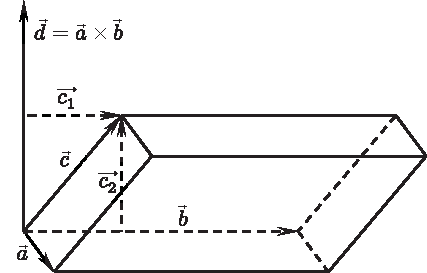
\includegraphics[width=0.9\linewidth]{picture/C-1/1.2/HHJ.pdf}
			\caption{外积的几何意义}
			\label{混合积}
		\end{minipage}
	\end{figure}
\end{enumerate}
\subsection{混合积}\index{HHJ@混合积}
\begin{enumerate}[1.]
			\setlength{\itemindent}{1.5em} 
	\setlength{\topsep}{0.01em}
	\setlength{\itemsep}{0.01em}
	\item {\color{dy2}几何表示}
	\begin{enumerate}[]
				\setlength{\itemindent}{1.5em} 
		\setlength{\topsep}{0.01em}
		\setlength{\itemsep}{0.01em}
		\item 两个向量$\overrightarrow{a},\overrightarrow{b}$的外积后与另一个向量$\overrightarrow{c}$内积后是一个数,记为
		\begin{equation}
			\left( \overrightarrow{a}\times\overrightarrow{b}\right) \cdot \overrightarrow{c}
		\end{equation}
		\item {\color{dy}几何意义}\label{混合积的几何意义}:$\left|\overrightarrow{a}\times\overrightarrow{b}\cdot \overrightarrow{c} \right|$代表的是分别以$\overrightarrow{a},\overrightarrow{b},\overrightarrow{c}$为邻边的平行六面体的体积. 如图\ref{混合积}.
	\end{enumerate}

	\item {\color{dy2}坐标表示}
	\begin{enumerate}[]
				\setlength{\itemindent}{1.5em} 
		\setlength{\topsep}{0.01em}
		\setlength{\itemsep}{0.01em}
		\item 设在仿射标架$[O,\overrightarrow{e_1},\overrightarrow{e_2},\overrightarrow{e_3}]$中$\overrightarrow{a},\overrightarrow{b},\overrightarrow{c}$的坐标分别为:$(a_1,a_2,a_3),(b_1,b_2,b_3),(c_1,c_2,c_3)$,则
		\begin{equation}
			\begin{aligned}
				(\overrightarrow{a} \times \overrightarrow{b})\cdot \overrightarrow{c}&=(a_1\overrightarrow{e_1}+a_2\overrightarrow{e_2}+a_3\overrightarrow{e_3})\times (b_1\overrightarrow{e_1}+b_2\overrightarrow{e_2}+b_3\overrightarrow{e_3})\\
				&=\left( a_1b_2-a_2b_1\right)\cdot \left[\overrightarrow{e_1}\times \overrightarrow{e_2}\right]+\left(a_3b_1-a_1b_3\right)\cdot \left[\overrightarrow{e_3}\times \overrightarrow{e_1}\right]\\
				&\quad +\left(a_2b_3-a_3b_2\right)\cdot \left[\overrightarrow{e_2}\times \overrightarrow{e_3}\right]\cdot \left( c_1\overrightarrow{e_1}+c_2\overrightarrow{e_2}+c_3\overrightarrow{e_3}\right) \\
				&=[(a_1b_2-a_2b_1)c_3+(a_3b_1-a_1b_3)c_2+(a_2b_3-a_3b_2)c_1]\,\,(\overrightarrow{e_1}\times \overrightarrow{e_2}\cdot \overrightarrow{e_3})\\
				&=\begin{array}{|ccc|}
					a_1 & a_2 & a_3 \\
					b_1 & b_2 & b_3 \\
					c_1 & c_2 & c_3
				\end{array}\cdot (\overrightarrow{e_1}\times \overrightarrow{e_2}\cdot \overrightarrow{e_3})
			\end{aligned}
		\end{equation}
		\addentheorem[混合积表示]{设在仿射标架$[O,\overrightarrow{e_1},\overrightarrow{e_2},\overrightarrow{e_3}]$中$\overrightarrow{a},\overrightarrow{b},\overrightarrow{c}$的坐标分别为:$(a_1,a_2,a_3)$,\\
			$(b_1,b_2,b_3),(c_1,c_2,c_3)$,则
			\begin{equation}
				\frac{(\overrightarrow{a} \times \overrightarrow{b})\cdot \overrightarrow{c}}{(\overrightarrow{e_1}\times \overrightarrow{e_2})\cdot \overrightarrow{e_3}}=
				\begin{array}{|ccc|}
					a_1 & a_2 & a_3 \\
					b_1 & b_2 & b_3 \\
					c_1 & c_2 & c_3
				\end{array}
			\end{equation}
			特别地,当仿射坐标系的基向量两两垂直时,即为直角坐标系时,混合积表达式可写为:
			\begin{equation}
				(\overrightarrow{a} \times \overrightarrow{b})\cdot \overrightarrow{c}=
				\begin{array}{|ccc|}
					a_1 & a_2 & a_3 \\
					b_1 & b_2 & b_3 \\
					c_1 & c_2 & c_3
				\end{array}
			\end{equation}
		}
	\end{enumerate}
	\item {\color{dy2}性质}
	\begin{equation}
		\left( \overrightarrow{a}\times \overrightarrow{b}\right) \cdot \overrightarrow{c}=\left( \overrightarrow{b}\times \overrightarrow{c}\right) \cdot \overrightarrow{a}=\left( \overrightarrow{c}\times\overrightarrow{a}\right) \cdot \overrightarrow{b}=\overrightarrow{a}\cdot \left( \overrightarrow{b}\times \overrightarrow{c}\right) .
	\end{equation}
	即混合积的轮换式相等$(a,b,c)=(b,c,a)=(c,a,b)$,任意两个向量交换顺序都要加上负号. \\
\end{enumerate}
\subsection{射影和分量}
\tdefination[射影]
\hspace*{0.3cm} 若向量$\overrightarrow{a}=\overrightarrow{ a_1}+\overrightarrow{a_2}$,其中$\overrightarrow{a_1}\parallel \overrightarrow{e},\overrightarrow{ a_2}\perp \overrightarrow{e},\overrightarrow{e}$是单位向量,则称$\overrightarrow{a_1}$是在$\overrightarrow{e}$方向上的{\color{dy}内射影\index{SY@射影!NSY@内射影}(简称射影\index{SY@射影!SY@射影})},也称{\color{dy}投影向量\index{SY@射影!TYXL@投影向量}};称$\overrightarrow{a_1}$是在$\overrightarrow{e}$方向$\overrightarrow{e}$下的{\color{dy}外射影\index{SY@射影!WSY@外射影}}.

\begin{figure}[h]
	\begin{minipage}{0.65\linewidth}
		\defination[分量]
		\hspace*{0.3cm} 若向量$\overrightarrow{a_1}$是$\overrightarrow{a}$在方向$\overrightarrow{e}$(单位向量)上的内射影,则存在唯一的实数$\lambda $使得$\overrightarrow{a_1}=\lambda \overrightarrow{e}$,这个实数$\lambda $被称为$\overrightarrow{a}$在方向$\overrightarrow{e}$上的{\color{dy}分量\index{SY@射影!FL@分量}(也称投影\index{SY@射影!TY@投影})},记作$\Pi_{\overrightarrow{e}}\overrightarrow{a}$,其值为
		\begin{equation}
			\Pi_ {\overrightarrow{e}}\overrightarrow{a}=|\overrightarrow{a}|\cos \left\langle \overrightarrow{a},\overrightarrow{e}\right\rangle=\frac{\overrightarrow{a}\cdot \overrightarrow{e}}{|\overrightarrow{e}|}=\overrightarrow{a}\cdot \overrightarrow{e}.
		\end{equation}
		
	\end{minipage}
	\hfill
	\begin{minipage}{0.35\linewidth}
		\centering
		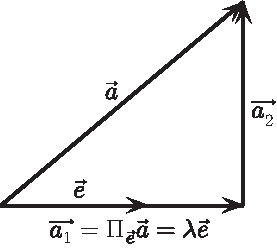
\includegraphics[width=0.7\linewidth]{picture/C-1/1.2/TY.pdf}
		\caption{向量的射影}
		\label{TY}
	\end{minipage}
\end{figure}
这里特别要注意的是:射影(投影向量)是矢量,而分量(投影)才是标量!\\
\vspace*{-2em}
\subsection{二重外积}\index{ECWJ@二重外积}

\ttheorem[二重外积公式]
对任意向量$\overrightarrow{a},\overrightarrow{b},\overrightarrow{c},$有
\begin{equation}
	\overrightarrow{a}\times\left( \overrightarrow{b}\times\overrightarrow{c}\right) =\left( \overrightarrow{a}\cdot \overrightarrow{c}\right)\overrightarrow{b}-\left( \overrightarrow{a}\cdot  \overrightarrow{b}\right)\overrightarrow{c}.  
	\label{二重外积}
\end{equation}
\qquad  二重外积公式\eqref{二重外积}表明$\overrightarrow{a}\times\left( \overrightarrow{b}\times\overrightarrow{c}\right)$是向量$\overrightarrow{b},\overrightarrow{c}$的线性组合,即$\overrightarrow{a}\times\left( \overrightarrow{b}\times\overrightarrow{c}\right)$与向量$\overrightarrow{b},\overrightarrow{c}$共面. 

\section{向量共线、共面的判断条件汇总}
\subsection{向量或三点共线的通用判定条件}\index{SDGX@三点共线}
\begin{enumerate}[1.]
	\setlength{\itemindent}{0em}
	\setlength{\topsep}{0.01em}
	\setlength{\itemsep}{0.01em}
	\item {\color{dy2}几何表示}
	
	\enbelowtheorem[共线定理1]
	\quad $\overrightarrow{a},\overrightarrow{b}$共线的充分必要条件是存在不全为$0$的实数$\lambda,\mu $,使得
	\begin{equation}
		\lambda \overrightarrow{a}+\mu \overrightarrow{b}=\overrightarrow{0}
		\label{gx1}
	\end{equation}
	{\color{dy} 而$\overrightarrow{a},\overrightarrow{b}$不共线的充分必要条件是式\eqref{gx1}中$\lambda=\mu=0 $.}
	
	\addentheorem[共线定理2]
	\quad $\overrightarrow{a},\overrightarrow{b}$共线的充分必要条件是存在实数$\lambda $,使得
	\begin{equation}
		\overrightarrow{a}=\lambda \overrightarrow{b}
		\label{gx2}
	\end{equation}
	\qquad {\color{dy}注:式\eqref{gx1},\eqref{gx2}本质是线性组合和线性相关性(式\eqref{线性相关})的具体应用. }
	
	\addentheorem[共线定理3]
	\quad $\overrightarrow{a},\overrightarrow{b}$共线的充分必要条件是
	\begin{equation}
		\overrightarrow{a}\times\overrightarrow{b}=\overrightarrow{0}
	\end{equation}
	
	\item {\color{dy2}坐标表示}
	
	\enbelowtheorem[共线定理4]
	\quad 在三个点$A,B,C$所在平面上取一个仿射坐标系$[O;\overrightarrow{e_1},\overrightarrow{e_2}]$,设$A,B,C$的坐标分别是
	$$(a_1,a_2),(b_1,b_2),(c_1,c_2)$$
	则$A,B,C$三点共线的充分必要条件是
	\begin{equation}
		\begin{array}{|ccc|}
			a_1 & b_1 & c_1 \\
			a_2 & b_2 & c_2 \\
			1 & 1 & 1
		\end{array}=0
	\end{equation}
	
	\addentheorem[共线定理5]
	\quad 设仿射坐标系$[O;\overrightarrow{e_1},\overrightarrow{e_2},\overrightarrow{e_3}]$上的两个向量$\overrightarrow{a},\overrightarrow{b}$的坐标分别是$(a_1,a_2,a_3)$,\\$(b_1,b_2,b_3).$则$\overrightarrow{a},\overrightarrow{b}$共线的充分必要条件是
	\begin{equation}
		\begin{array}{|cc|}
			a_1 & b_1  \\
			a_2 & b_2 
		\end{array}=
		\begin{array}{|cc|}
			a_1 & b_1  \\
			a_3& b_3 
		\end{array}=
		\begin{array}{|cc|}
			a_2 & b_2  \\
			a_3 & b_3 
		\end{array}=0
	\end{equation}
\end{enumerate}

\subsection{向量或四点共面的通用判定条件}\index{SDGM@四点共面}
\begin{enumerate}[1.]
	\setlength{\itemindent}{0em}
	\setlength{\topsep}{0.01em}
	\setlength{\itemsep}{0.01em}
	\item {\color{dy2}几何表示}
	
	\enbelowtheorem[共面定理1]
	\quad $\overrightarrow{a},\overrightarrow{b},\overrightarrow{c}$共线的充分必要条件是存在不全为$0$的实数$k_1,k_2,k_3 $,使得
	\begin{equation}
		k_1\overrightarrow{a}+k_2\overrightarrow{b}+k_3\overrightarrow{c}=\overrightarrow{0}
		\label{gm1}
	\end{equation}
	{\color{dy} 而$\overrightarrow{a},\overrightarrow{b}$不共面的充分必要条件是式\eqref{gm1}中$k_1=k_2=k_3=0 $.}
	
	\newpage
	\addentheorem[共面定理2]
	\quad $\overrightarrow{a},\overrightarrow{b},\overrightarrow{c}$共面的充分必要条件是存在实数$\lambda ,\mu $,使得
	\begin{equation}
		\overrightarrow{c}=\lambda \overrightarrow{a}+\mu\overrightarrow{b}
		\label{gm2}
	\end{equation}
	{\color{dy}\qquad 注:式\eqref{gm1},\eqref{gm2}本质是线性组合和线性相关性(式\eqref{线性相关})的具体应用. }
	
	
	\addentheorem[共面定理3]
	\quad $\overrightarrow{a},\overrightarrow{b},\overrightarrow{c}$共面的充分必要条件是
	\begin{equation}
		\left( \overrightarrow{a}\times\overrightarrow{b}\right) \cdot \overrightarrow{c}=0
	\end{equation}
	
	\item {\color{dy2}坐标表示}
	
	\enbelowtheorem[共面定理4]
	\quad 设$\overrightarrow{a},\overrightarrow{b},\overrightarrow{c}$的仿射坐标分别为:
	$$(a_1,a_2,a_3),(b_1,b_2,b_3),(c_1,c_2,c_3)$$
	则$\overrightarrow{a},\overrightarrow{b},\overrightarrow{c}$共面的充分必要条件是
	\begin{equation}
		\begin{array}{|ccc|}
			a_1 & a_2 & a_3 \\
			b_1 & b_2 & b_3 \\
			c_1 & c_2 & c_3
		\end{array}=0
	\end{equation}
	
	
	\addentheorem[共面定理5]
	\quad 设四个点$A,B,C,D$的仿射坐标分别为:
	$$(x_1,y_1,z_1),(x_2,y_2,z_2),(x_3,y_3,z_3),(x_4,y_4,z_4)$$
	则点$A,B,C,D$共面的充分必要条件是
	\begin{equation}
		\begin{array}{|cccc|}
			x_1 & y_1 & z_1 & 1 \\
			x_2 & y_2 & z_2 & 1 \\
			x_3 & y_3 & z_3 & 1 \\
			x_4 & y_4 & z_4 & 1
		\end{array}=0
		\label{SDGM}
	\end{equation}
\end{enumerate} 
